%//==============================--@--==============================//%
\subsection{Máquina Assíncrona}

\noindent Um motor assíncrono (também designado por \textit{motor de indução}) recebe energia da rede elétrica e fornece energia mecânica a uma carga (também pode funcionar como gerador): é um \underline{conversor eletromecânico}.

\begin{figure}[H]
    \centering
    \begin{tikzpicture}[very thick,sc/.style={circle,draw,inner sep=1.5pt},scale=0.6]
         \begin{scope}
              \clip (4,0) arc(0:-360:4) (0,0) circle[radius=5cm];
              \fill[gray!50,even odd rule] circle[radius=5cm] circle[radius=4cm] 
               foreach \X in {1,...,6} {(\X*60:4) circle[radius=0.5cm]};
         \end{scope}
         
         \foreach \X [count=\Y starting from 0] in {A,B,C,A,B,C} { 
             \path(180-60*\Y:4) node[circle,draw, scale=0.6] (n\Y) {\X};
         }
         
         \foreach \Y in {0,...,4}{
            \draw[dashed,-{Stealth[bend]}] (180-72*\Y-5:3) arc(180-72*\Y-5:180-72*\Y-67:3);
            }
            
         \fill[gray!70] circle[radius=1.8cm];   
         \foreach \X in {1,...,20}{
            \draw (\X*18:2) circle[radius=0.12cm];
         }
         
         \draw (n1) -- (120:5.8) coordinate (aux) -- (-6.7,0|-aux)  node[sc,left] (c1){};
         \draw (n3) -- (0:5.8) |- ([yshift=8mm]c1.east)  node[sc,left] (c3){};
         \draw (n5) -- (-120:5.8) -| ([yshift=-8mm,xshift=5mm]c1.east)  
         -- ++(-0.5,0)node[sc,left] (c5){};
         \draw[decorate,decoration={brace,mirror,raise=2pt}] (c3.north west) -- (c5.south west)
          node[midway,left=3pt,align=right]{3 Phase\\ input};
         \draw (n0) -| (-5.8,-5.8) node[sc,fill] {} -- ++ (-1,0)
          node[left,sc,label=left:Common] (Common){};
         \draw (n4) -- (-60:5.6) coordinate(aux) -- (aux|-Common) node[sc,fill]{};
         \draw (n2) -- (60:5.6) coordinate(aux) -- (aux-|6,0) |- (Common);
    \end{tikzpicture}

    \caption{Motor de indução trifásico.}
\end{figure}

\noindent A máquina assíncrona trifásica é constituída por um estator (camada exterior) e um rotor (camada interior). Da aplicação de um sistema trifásico de tensões ao enrolamento do estator, resulta no entreferro um fluxo magnético girante, o qual induz no enrolamento do rotor uma f.e.m. Uma vez que o rotor está em curto circuito (rotor em gaiola) ou fechado através de circuito exterior (rotor bobinado), esta f.e.m. dá origem a correntes que circulam no rotor, \underline{produzindo um binário motor}.

\begin{minipage}[b]{0.275\linewidth}
   \begin{figure}[H]
        \centering
        \begin{tikzpicture}[scale=2, transform shape]
        
            \def\samples{200}
            
            % Draw sine waveforms
            \draw[domain=pi:2*pi, samples=\samples] plot (\x,{sin(\x r)});
            \draw[domain=pi:2*pi, samples=\samples] plot (\x,{sin((\x - 2*pi/3) r)});
            \draw[domain=pi:2*pi, samples=\samples] plot (\x,{sin((\x + 2*pi/3) r)});
            
            % Function to draw rotating field representation
            \newcommand\rotatingfield[3]{
                \begin{scope}[shift={(#1,#2)}]
                    \clip (0.4,0) arc(0:-360:0.4) (0,0) circle[radius=0.5cm];
                    \fill[gray!50,even odd rule] circle[radius=0.5cm] circle[radius=0.4cm] 
                    foreach \X in {1,...,6} {(\X*60:0.4) circle[radius=0.07cm]};
            
                \end{scope}
                \begin{scope}[shift={(#1,#2)}]
                     \foreach \X [count=\Y starting from 0] in {A,B,C,A,B,C} { 
                         \path(180-60*\Y:0.4) node[circle,draw,scale=0.15] (n\Y) {\X};
                    }
                    \fill[gray!70] circle[radius=0.16cm];   
                    \foreach \X in {1,...,20}
                    {\draw (\X*18:0.2) circle[radius=0.018cm];}
            
                    % Draw an arrow at the specified angle
                    \draw[blue,-{Stealth[length=3.5pt]}] (0,0) -- (#3:0.14);
                \end{scope}
            }
            
            % Draw vertical dotted lines at intersections and motor direction rotating fields
            \draw[dotted, thin] (5.7596,-1.1) -- (5.7596,1.5);
            \rotatingfield{5.7596}{2}{-60} % Example angle of 45 degrees
            \draw[dotted, thin] (3.6652,-1.1) -- (3.6652,1.5);
            \rotatingfield{3.6652}{2}{60} % Example angle of -30 degrees
            \draw[dotted, thin] (4.7124,-1.1) -- (4.7124,1.5);
            \rotatingfield{4.7124}{2}{0} % Example angle of 90 degrees
            
            % Draw y-axis
            \draw[-{Stealth[length=2.0pt]}] (pi,-1.1) -- (pi,1.1);
            \draw (pi-0.15,0.85) node[circle,draw,scale=0.2] {C};
            \draw (pi-0.15,-0.05) node[circle,draw,scale=0.2] {A};
            \draw (pi-0.15,-0.85) node[circle,draw,scale=0.2] {B};
        
        \end{tikzpicture}
    \end{figure} 
\end{minipage}\hfill
\begin{minipage}[b]{0.53\linewidth}
 \noindent \textbf{No motor de indução:}
 \begin{itemize}
     \item A energia AC fornecida ao estator do motor cria um campo magnético que roda em sincronismo com as oscilações AC.
     \item O rotor gira a uma velocidade um pouco mais lenta do que o campo do estator. O campo magnético do estator está, portanto, a mudar ou a rodar relativamente ao rotor.
     \item Isto induz uma corrente oposta no rotor, que é efetivamente a segunda bobina do motor.
     \item O fluxo magnético rotativo induz correntes nas bobinas do rotor, de forma semelhante às correntes induzidas nas bobinas secundárias de um transformador.
 \end{itemize}
\end{minipage}

\vspace{1em}
\noindent Estando o motor em repouso, as correntes no rotor têm uma frequência igual à da tensão de alimentação; à medida que o rotor acelera, por ação do binário motor, aquela frequência vai diminuindo. 

Se o motor estiver em vazio, a frequência e a amplitude das correntes no rotor são muito próximas de zero. Estando o motor a acionar um carga mecânica que oferece um binário resistente, a frequência e a resultante amplitude das \textit{correntes rotóricas} terão um valor correspondente ao binário motor necessário para estabilizar a marcha da máquina.

\begin{mdframed}
    Em termos de \textbf{balanço energético}, a energia recebida da rede elétrica é transferida para o rotor por efeito indutivo, deduzida das perdas no ferro do estator e no cobre do enrolamento respetivo. Subtraindo as perdas no rotor e as perdas mecânicas, obtém-se a \underline{potência mecânica final fornecida à carga}.
\end{mdframed}

%//==============================--@--==============================//%
\subsubsection{Modelo Matemático e Esquema Equivalente}

Definimos a \textit{velocidade síncrona} do rotor como:
$$
    n_s = \frac{60 f}{p}\; [\text{rpm}] \implies \omega_s = n_s \frac{2\pi}{60} = \frac{2\pi f}{p}\; [\text{rad/s}]
$$
em que $f$ é a frequência da tensão de alimentação e $p$ o número de pares de pólos do enrolamento do estator.

A diferença entre a velocidade síncrona e a velocidade de rotação do rotor ($n_r$), expressa em em p.u. (ou percentagem) na base da primeira, designa-se por \textit{escorregamento} (ou \textit{deslizamento}):
$$
    s = \frac{n_s - n_r}{n_s} = \frac{\omega_s - \omega_r}{\omega_s}
$$
onde $\omega_s$ e $\omega_r$ são as velocidades angulares respetivas. O escorregamento tem um valor muito baixo em vazio, e vai aumentando à medida que a carga aumenta.

\vspace{0.5em}
\hrule
\vspace{0.5em}
\noindent Podemos modelar a máquina síncrona através de um esquema equivalente em T, à semelhança do que se faz para o transformador (ver Apêndice X para mais detalhes):

\vspace{-0.75em}
\begin{figure}[H]
    \centering
    \scalebox{0.915}{%
    \begin{circuitikz}[american,>=latex]
        \ctikzset{inductor=cute}    
        \ctikzset{inductors/coils=4}
        \ctikzset{bipoles/resistor/height=0.25}
        \ctikzset{bipoles/resistor/width=0.5}
        \ctikzset{resistors/zigs=4}
        
        % circuit
        \draw 
            (0,0) to[short,*-] 
            (1,0) to[R=$R_s$]
            (2.5,0) to[L=$jX_s$] 
            (4,0) to[short,-*] (5,0)
            ;

        \draw
            (5,0) to[short,-*] 
            (5,-1) to[short] (4.5,-1) to[short] (5.5,-1) 
            ;

        \draw
            (4.5,-1) to[R,l_=$G_m$] (4.5,-2.5)
            ;
            
        \draw
            (5.5,-1) to[L=$jB_m$] (5.5,-2.5)
            ;

        \draw
            (5,-2.5) to[short] (4.5,-2.5) to[short] (5.5,-2.5)
            to[short] (5,-2.5) to[short,*-] (5,-3.5)
            ;

        \draw
            (5,0) to[short] 
            (6,0) to[short] %to[R=$R_r$]
            (7.5,0) to[L=$jX_r$]
            (9,0) to[short] 
            (10,0) to[R,l_=$\displaystyle \frac{R_r}{s}$,*-] (10,-2.5)
            ;

        \draw (0,-3.5) to[short,*-] (11,-3.5) to[short] (11, -1.25);
        \draw[->] (11,-1.25) -- (10.3,-1.25);

        % labels and arrows
        \draw[->] (0,-0.25) -- (0,-3.25) node[midway,left] {$\mathbf{V}_s$};
        \draw[->] (4.45,0) -- (4.5,0) node[midway,above] {$\mathbf{I}_s$};
        \draw[->] (5,-0.5) -- (5,-0.6) node[midway,right] {$\mathbf{I}_m$};
        \draw[->] (5.7,0) -- (5.75,0) node[midway,above] {$\mathbf{I}_r$};

        \draw[->] (7.25,-0.25) -- (7.25,-3.25) node[midway,right] {$\mathbf{E}_s$};
        
    \end{circuitikz}}
    \caption{Esquema equivalente em T da máquina assíncrona.}
    \label{fig:esquema-T-maquina-assincrona}
\end{figure}

\noindent A potência transferida para o rotor corresponde à potência consumida na resistência fictícia ($R_r/s$), que é igual à potência fornecida pela rede menos as perdas no estator e no circuito magnético:
$$
    P_r = 3\frac{R_r}{s} I^2_r   
$$
A potência mecânica é igual à potência $P_r$ menos as perdas no rotor:
$$
    P_M = P_r - 3R_r I^2_r = 3 \frac{1-s}{s} R_r I^2_r
$$
O esquema equivalente pode ser modificado de forma a modelar a carga mecânica:

\begin{minipage}[c]{0.525\linewidth}
\begin{figure}[H]
    \centering
    \scalebox{0.915}{%
    \begin{circuitikz}[american,>=latex]
        \ctikzset{inductor=cute}    
        \ctikzset{inductors/coils=4}
        \ctikzset{bipoles/resistor/height=0.25}
        \ctikzset{bipoles/resistor/width=0.5}
        \ctikzset{resistors/zigs=4}
        
        % circuit
        \draw 
            (2.5,0) to[short,*-*] (5,0)
            ;

        \draw
            (5,0) to[short,-*] 
            (5,-1) to[short] (4.5,-1) to[short] (5.5,-1) 
            ;

        \draw
            (4.5,-1) to[R,l_=$G_m$] (4.5,-2.5)
            ;
            
        \draw
            (5.5,-1) to[L=$jB_m$] (5.5,-2.5)
            ;

        \draw
            (5,-2.5) to[short] (4.5,-2.5) to[short] (5.5,-2.5)
            to[short] (5,-2.5) to[short,*-] (5,-3.5)
            ;

        \draw
            (5,0) to[short] 
            (6,0) to[R, l=$R_s+R_r$]
            (8,0) to[L, l=$j(X_s+X_r)$]
            (9.5,0) to[short] 
            (10.5,0) to[R,l_=$\displaystyle \frac{1-s}{s}R_r$,*-] (10.5,-2.5)
            ;

        \draw (2.5,-3.5) to[short,*-] (11.5,-3.5) to[short] (11.5, -1.25);
        \draw[->] (11.5,-1.25) -- (10.75,-1.25);

        % labels and arrows
        \draw[->] (2.5,-0.25) -- (2.5,-3.25) node[midway,left] {$\mathbf{V}_s$};
        \draw[->] (4.45,0) -- (4.5,0) node[midway,above] {$\mathbf{I}_s$};
        \draw[->] (5,-0.5) -- (5,-0.6) node[midway,right] {$\mathbf{I}_m$};
        \draw[->] (5.7,0) -- (5.75,0) node[midway,above] {$\mathbf{I}_r$};
        
    \end{circuitikz}}
    \caption{Esquema equivalente em L da máquina assíncrona.}
    \label{fig:esquema-L-maquina-assincrona}
\end{figure}
\end{minipage}\hfill
\begin{minipage}[c]{0.4\linewidth}
    Podemos deslocar o ramo longitudinal de modo a obter o esquema equivalente em L. No entanto, $\mathbf{I}_m$ é maior neste contexto (relativamente ao transformador), o que torna o esquema numa aproximação mais grosseira.
    $$
        \left\{
        \begin{aligned}
            \mathbf{I}_r &= \frac{\mathbf{V}_s}{R_s + R_r/s + j(X_s + X_r)} \\
            \mathbf{I}_m &= (G_m + jB_m) \mathbf{V}_s
        \end{aligned}\right.
    $$
    $$
        \mathbf{I}_s = \mathbf{I}_m + \mathbf{I}_r
    $$
\end{minipage}

\vspace{0.5em}
\noindent A potência perdida é dada por
$$
    \therefore P_s = 3G_m V^2_s + 3 \left(R_s + \frac{R_r}{s} \right) I^2_r
$$
Donde resulta o rendimento:
$$
    \eta = \frac{P_M}{P_s} = \frac{(1-s)/s \cdot R_r I^2_r}{3G_m V^2_s + 3(R_s + R_r/s) I^2_r}
$$

\begin{mdframed}
    \noindent \textbf{Nota}: O motor assíncrono representa uma carga indutiva para a rede de alimentação com
    $$
        Q_s = -3B_m V^2_s + 3(X_s + X_r) I^2_r
    $$
\end{mdframed}

%//==============================--@--==============================//%
\subsubsection{Binário e Característica Binário-Velocidade}

Para além da potência, interessa calcular o binário:
$$
    T = \frac{P_M}{\omega_r} = \frac{P_M}{\omega_s (1-s)} = \frac{3 R_r I^2_r}{s \omega_s}
$$
Como $I^2_r = V^2_s/[(R_s + R_r)^2 + (X_s + X_r)^2]$, temos que:
$$
    T = \frac{3 V^2_s}{\omega_s} \frac{R_r}{(R_s + R_r)^2 + (X_s + X_r)^2}
$$
A região de funcionamento como motor corresponde a $s>0$ ou seja, a velocidade de rotação é menor que a do sincronismo; o funcionamento como gerador é caracterizado por $s<0$, uma vez que neste caso $\omega_r>\omega_s$.

\vspace{-0.5em}
\begin{minipage}[c]{.4\linewidth}
\begin{figure}[H]
    \centering
    \scalebox{0.95}{%
        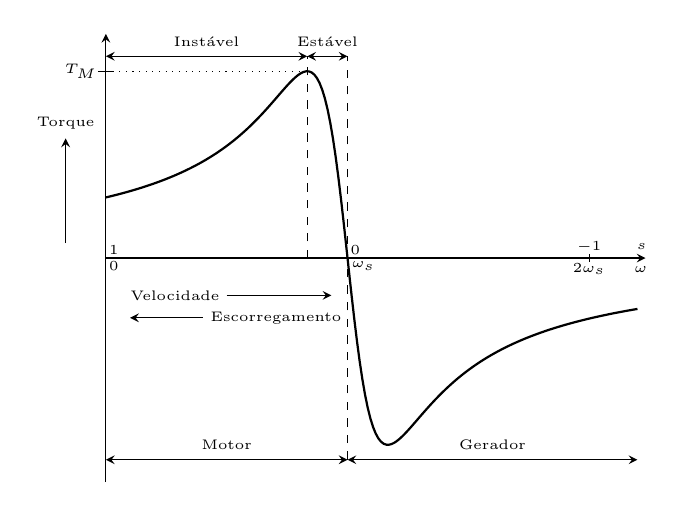
\begin{tikzpicture}[>=stealth]
            \begin{axis}[
                axis y line=left,
                axis x line=middle,
                xmax=3.7, 
                ymax=3, 
                ymin=-3,
                legend pos=north west,
                ticks=none,
                clip mode=individual
            ]
        
            % The torque-slip curve
            \addplot[black, thick, domain=-3:3.6, samples=200] {-x/(0.4*x^2 + 0.1)};
        
            % Vertical dashed line 
            \draw[dashed, black] (axis cs:-0.5,0) -- (axis cs:-0.5,2.7);
            \draw[dashed, black] (axis cs:0,-2.7) -- (axis cs:0,2.7);
        
            % horizontal dotted line 
            \draw[dotted, black] (axis cs:-3,2.5) -- (axis cs:-0.5,2.5);
            
            % Arrows indicating stable and unstable regions
            \draw[<->, thin] (axis cs:-3,2.7) -- (axis cs:-0.5,2.7) node[midway, above, font=\tiny] {Instável};
            \draw[<->, thin] (axis cs:-0.5,2.7) -- (axis cs:0,2.7) node[midway, above, font=\tiny] {Estável};
            
            % Regions
            \draw[<->, thin] (axis cs:-3,-2.7) -- (axis cs:0,-2.7) node[midway, above, font=\tiny] {Motor};
            \draw[<->, thin] (axis cs:0,-2.7) -- (axis cs:3.6,-2.7) node[midway, above, font=\tiny] {Gerador};
        
            % Manual tick marks
            \draw[black] (axis cs:-3.1,2.5) -- (axis cs:-2.9,2.5) node[left=0.9mm,font=\tiny] {$T_M$};
            \draw[black] (axis cs:3,-0.05) -- (axis cs:3,0.05);
            
            % Labels
            \node[yshift=-1mm,xshift=1mm,font=\tiny] at (-3,0) {$0$};
            \node[yshift=1mm,xshift=1mm,font=\tiny] at (-3,0) {$1$};
            
            \node[yshift=-1mm,xshift=2mm,font=\tiny] at (0,0) {$\omega_s$};
            \node[yshift=1mm,xshift=1mm,font=\tiny] at (0,0) {$0$};
        
            \node[yshift=-1.4mm,xshift=0mm,font=\tiny] at (3,0) {$2\omega_s$};
            \node[yshift=1.4mm,xshift=0mm,font=\tiny] at (3,0) {$-1$};
        
            \node[yshift=-1.5mm,xshift=-0.1mm,font=\tiny] at (3.65,0) {$\omega$};
            \node[yshift=1.5mm,font=\tiny] at (3.65,0) {$s$};
        
            % rando arrows
            \draw[->, thin] (axis cs:-3.5,0.2) -- (axis cs:-3.5,1.6) node[above, font=\tiny] {Torque};
            \draw[->, thin] (axis cs:-1.5,-0.5) -- (axis cs:-0.2,-0.5) node[left=13mm, font=\tiny] {Velocidade};
            \draw[->, thin] (axis cs:-1.8,-0.8) -- (axis cs:-2.7,-0.8) node[right=9mm, font=\tiny] {Escorregamento};
            \end{axis}
        \end{tikzpicture}
    }
    \caption{Característica binário-velocidade}
\end{figure}
\end{minipage}\hfill
\begin{minipage}[c]{.5\linewidth}
    O binário máximo pode calcular-se após uma simples análise da equação em ordem a $s$:
    $$
        \begin{aligned}
            s_{T_{max}} &= \frac{R_r}{\sqrt{R_s^2 + (X_s + X_r)^2}} \\
            T_{max} &= \frac{3V^2_s}{2R_r} \frac{1}{R_s + \sqrt{R_s^2 + (X_s + X_r)^2}}
        \end{aligned}
    $$
\end{minipage}

\vspace{0.5em}
\noindent O binário de arranque, com $s=1$, é dado por:
$$
    T_{arr} = \frac{3V^2_s}{\omega_s} \frac{R_r}{(R_s + R_r)^2 + (X_s + X_r)^2}
$$
E a corrente de arranque é
$$
    \mathbf{I}_{arr} = \frac{\mathbf{V}_s}{R_s + R_r + j(X_s + X_r)}
$$
Queremos reduzir esta corrente, quando $\omega_r = 0$ e $s=1$, especialmente em motores de potência elevada, mas isto resulta na diminuição de $T_{arr}$, o que se pode revelar problemático para certas cargas mecânicas.
%//==============================--@--==============================//%
\subsubsection{Representação em Valores p.u.}

No contexto da máquina assíncrona, normalmente especifica-se a tensão e corrente nominais, e a potência mecânica. Tomam-se os valores da tensão e da corrente nominais como base, calcula-se a potência aparente de base:
$$
    S_b = \sqrt{3} V_b I_b
$$
Tomando como valor base para a velocidade angular:
$$
    \omega_b = \omega_s = \frac{2\pi f}{p} \implies \omega_r = 1-s
$$
As restantes equações ficam
$$
        P_r = \frac{R_r}{s} I^2_r  \qquad\rightarrow\qquad P_M = P_r - R_r I^2_r = \frac{1-s}{s} R_r I^2_r
$$
$$
    \left\{
    \begin{aligned}
        P_s &= G_m V^2_s + (R_s + R_r/s) I^2_r \\
        Q_s &= -B_m V^2_s + (X_s + X_r) I^2_r
    \end{aligned}\right.
$$

\vspace*{0.5em}
$$
        T = \frac{P_M}{\omega_r} = \frac{P_M}{1-s} = V^2_s \frac{R_r/s}{(R_s + R_r/s)^2 + (X_s + X_r)^2}
$$
$$
    \left\{
    \begin{aligned}
        T_{arr} &= V^2_s \frac{R_r}{(R_s + R_r)^2 + (X_s + X_r)^2} \\
        T_{max} &= \frac{V^2_s}{2} \frac{1}{R_s + \sqrt{R^2_s + (X_s + X_r)^2}}
    \end{aligned}\right.
$$

%//==============================--@--==============================//%
\clearpage
\subsubsection{Análise da Máquina Assíncrona}
%//==============================--@--==============================//%
\paragraph{Ensaio em Vazio}

Semelhante ao ensaio que se faz no transformador para determinar os parâmetros transversais. Aplica-se a tensão nominal ao estator da máquina sem qualquer carga mecânica no veio ($s \approx 0$).

\begin{figure}[H]
    \centering
    \ctikzset{bipoles/resistor/height=0.20}
    \ctikzset{bipoles/resistor/width=0.5}
    \begin{circuitikz}[=>stealth,american]
        % circuito
        \draw (0,0) to [short, *-] (3,0);

        \draw (3,-0.5) to [short] (3,0);
        \draw (2.5,-0.5) to [short] (3.5,-0.5);
        \draw (2.5,-0.5) to [R, l_=$G_m$] (2.5,-2.5);
        \draw (3.5,-0.5) to [cute inductor, l=$jB_m$] (3.5,-2.5);
        \draw (2.5,-2.5) to [short] (3.5,-2.5);
        \draw (3,-2.5) to [short] (3,-3);

        \draw (3,-3) to [short] (0,-3) node[circ] {};

        % tensão e corrente de magnetização
        \draw[->] (0,-0.25) -- (0,-2.75) node[midway,left] {$V_n$};
        \draw[->] (3,-0.25) -- (3,-0.30) node[midway,right] {$I_m$};
    \end{circuitikz}
    \caption{Esquema equivalente do ensaio em vazio.}
    \label{fig:ensaio-vazio-maq-async}
\end{figure}

\vspace{-0.5em}
\noindent Os valores de $G_m$ e $B_m$ obtêm-se igualmente das medidas da tensão aplicada $V_n$, corrente de magnetização $I_m$ e potência de perdas em vazio $P_0$:
$$
    G_m = \frac{P_0}{V_n^2} 
    \mkern48mu
    B_m = -\sqrt{\left(\frac{I_m}{V_n}\right)^2-G_m^2}
$$

%//==============================--@--==============================//%
\paragraph{Ensaio com Rotor Bloqueado}

Neste ensaio o rotor é mantido parado ($s \approx 1$), o que resulta numa resistência $R (1-s)/s$ nula. O esquema equivalente é igual ao do ensaio em curto-circuito no transformador. Aplica-se uma tensão reduzida ao estator até a corrente atingir o valor nominal.
$$
    \left\{\begin{aligned}
        V_{cc} &= Z_{cc} I_n\\
        I_n &= 1.0\; \text{p.u.}
    \end{aligned}\right.\quad\rightarrow\quad
    \boxed{V_{cc} = Z_{cc}} 
$$
\noindent Para decompor a impedância de curto-circuito nas suas componentes resistiva e reativa, é preciso conhecer a potência $P_{cc}$:
$$
    R_t = \dfrac{P_{cc}}{I_n^2} = P_{cc}\qquad
    Z_{cc} = V_{cc} = \sqrt{R_t^2 + X_t^2}\qquad
    X_t = \sqrt{Z_t^2 - R_t^2}
$$
%//==============================--@--==============================//%
\subsubsection{Funcionamento como Gerador}

A máquina assíncrona, além das suas funções habituais, também pode operar como gerador, sendo especialmente utilizada em centrais de baixa potência alimentadas por fontes renováveis. Ao contrário da máquina síncrona, que possui um sistema de excitação próprio, a máquina assíncrona requer uma corrente de magnetização do exterior, normalmente fornecida pela rede elétrica.

Quando funciona como gerador, a máquina assíncrona tem certas características específicas. Recebe energia mecânica (de um motor, por exemplo) e entrega energia elétrica à rede. No entanto, mesmo fornecendo energia ativa, continua a absorver energia reativa, o que exige compensação através de uma bateria de condensadores. Dependendo das condições, esta bateria pode ser ajustada para que o gerador assíncrono também forneça energia reativa.


\begin{mdframed}
    \vspace{1.5cm}
    \hfil (Adicionar imagem)
    \vspace{1.5cm}
\end{mdframed}


\noindent Um ponto interessante é que um gerador assíncrono pode auto-excitar-se quando está em vazio e ligado a um condensador, dependendo da capacitância do condensador. Na prática, a ligação deste gerador à rede pode ser feita de duas formas distintas: rodando a uma velocidade próxima da nominal ou utilizando uma bateria de condensadores de valor apropriado. A segunda opção evita sobre-correntes indesejadas.

%//==============================--@--==============================//%